\documentclass[a5paper, 10pt]{article}

% Текст
\usepackage[utf8]{inputenc} % UTF-8 кодировка
\usepackage[russian]{babel} % Русский язык
\usepackage{indentfirst} % красная строка в первом параграфе в главе
% Отображение страниц
\usepackage{geometry} % размеры листа и отступов
\usepackage{listings}
\usepackage{color}

\geometry{
	left=12mm,
	top=25mm,
	right=15mm,
	bottom=17mm,
	marginparsep=0mm,
	marginparwidth=0mm,
	headheight=10mm,
	headsep=7mm,
	nofoot}
\usepackage{afterpage,fancyhdr} % настройка колонтитулов
\pagestyle{fancy}
\fancypagestyle{style}{ % создание нового стиля style
	\fancyhf{} % очистка колонтитулов
	\fancyhead[LO, RE]{Лаб. работа № 1 } % название документа наверху
	\fancyhead[RO, LE]{Формы представления линейных динамических систем} % название section наверху
	\fancyfoot[RO, LE]{\thepage} % номер страницы справа внизу на нечетных и слева внизу на четных
	\renewcommand{\headrulewidth}{0.25pt} % толщина линии сверху
	\renewcommand{\footrulewidth}{0pt} % толцина линии снизу
}
\fancypagestyle{plain}{ % создание нового стиля plain -- полностью пустого
	\fancyhf{}
	\renewcommand{\headrulewidth}{0pt}
}
\fancypagestyle{title}{ % создание нового стиля title -- для титульной страницы
	\fancyhf{}
	\fancyhead[C]{{\footnotesize
			Министерство образования и науки Российской Федерации\\
			Федеральное государственное автономное образовательное учреждение высшего образования
	}}
	\fancyfoot[C]{{\large 
			Санкт-Петербург \\2024
	}}
	\renewcommand{\headrulewidth}{0pt}
}

% Математика
\usepackage{amsmath, amsfonts, amssymb, amsthm} % Набор пакетов для математических текстов
%\usepackage{dmvnbase} % мехматовский пакет latex-сокращений
\usepackage{cancel} % зачеркивание для сокращений
% Рисунки и фигуры
\usepackage[pdftex]{graphicx} % вставка рисунков
\usepackage{wrapfig, subcaption} % вставка фигур, обтекая текст
\usepackage{caption} % для настройки подписей
\captionsetup{figurewithin=none,labelsep=period, font={small,it}} % настройка подписей к рисункам
% Рисование
\usepackage{tikz} % рисование
\usepackage{circuitikz}
\usepackage{pgfplots} % графики
% Таблицы
\usepackage{multirow} % объединение строк
\usepackage{multicol} % объединение столбцов
% Остальное
\usepackage[unicode, pdftex]{hyperref} % гиперссылки
\usepackage{enumitem} % нормальное оформление списков
\setlist{itemsep=0.15cm,topsep=0.15cm,parsep=1pt} % настройки списков
% Теоремы, леммы, определения...
\theoremstyle{definition}
\newtheorem{Def}{Определение}
\newtheorem*{Axiom}{Аксиома}
\theoremstyle{plain}
\newtheorem{Th}{Теорема}
\newtheorem{Lem}{Лемма}
\newtheorem{Cor}{Следствие}
\newtheorem{Ex}{Пример}
\theoremstyle{remark}
\newtheorem*{Note}{Замечание}
\newtheorem*{Solution}{Решение}
\newtheorem*{Proof}{Доказательство}
% Свои команды
\newcommand{\comb}[1]{\left[\hspace{-4pt}\begin{array}{l}#1\end{array}\right.\hspace{-5pt} } % совокупность уравнений
% Титульный лист
\usepackage{csvsimple-l3}
\newcommand*{\titlePage}{
	\thispagestyle{title}
	\begingroup
	\begin{center}
		%		{\footnotesize
			%			Министерство образования и науки Российской Федерации\\
			%			Федеральное государственное автономное образовательное учреждение высшего образования
			%		}
		%		
		\vspace*{6ex}
		
		{\small
			САНКТ-ПЕТЕРБУРГСКИЙ НАЦИОНАЛЬНЫЙ ИССЛЕДОВАТЕЛЬСКИЙ УНИВЕРСИТЕТ ИТМО	
		}
		
		\vspace*{2ex}
		
		{\normalsize
			Факультет систем управления и робототехники
		}
		
		\vspace*{15ex}
		
		{\Large \bfseries 
			Лабораторная работа № 1
		}
\vspace*{2ex}
	{\Large \bfseries 
			
<<Формы представления линейных динамических систем>>
		}
\vspace*{2ex}
		
		{\normalsize
			по дисциплине <<Линейные системы автоматического управления>>
		}
\vspace*{2ex}
	{\Large \bfseries 
			
Вариант 27
		}

	\end{center}
	\vspace*{20ex}
	\begin{flushright}
		{\large 
			\underline{Студент}: группа \textbf{R3338}\\
			\begin{flushright}
				\textbf{Нечаева А. А.}\\
			\end{flushright}
		}
		
		\vspace*{5ex}
		
		{\large 
			\underline{Преподаватель}: \textit{Пашенко Артем Витальевич}
		}
	\end{flushright}	
	\newpage
	\setcounter{page}{1}
	\endgroup}

\begin{document}
	\titlePage
	\pagestyle{style}
\newpage

ДОБАВИТЬ СТРАНИЦУ СОДЕРЖАНИЕ

\section{Задание. Одноканальная система}
\subsection{Математическая модель}
Возьмем коэффициенты $a_2 = 9$, $a_1 = 23$, $a_0 = 15$, $b_2 = 14$, $b_1 = 6$ и $b_0 = 16$. Рассмотрим математическую модель в форме дифференциального уравнения
\begin{equation}
\dddot{y} + 9\ddot{y} + 23 \dot{y} + 15 y = 14 \ddot{u} + 6 \dot{u} + 16 u
\end{equation}

Перепишем с применением оператора дифференцирования
\begin{equation}
p^3[y] + 9p^2[y] + 23 p[y] + 15 y = 14 p^2[u] + 6 p[u] + 16 u
\end{equation}
Теперь выразим выходной сигнал $y$
\begin{multline}
p^3[y] = 14 p^2[u] + 6 p[u] + 16 u - 9p^2[y] - 23 p[y] - 15 y  \Leftrightarrow \\
 \Leftrightarrow y = \frac{1}{p^3} \left[ 14 p^2[u] + 6 p[u] + 16 u - 9p^2[y] - 23 p[y] - 15 y \right] = \\
= 14 \frac{1}{p}[u] + 6 \frac{1}{p^2}[u] + 16 \frac{1}{p^3}[u] - 9 \frac{1}{p}[y] - 23 \frac{1}{p^2}[y] - 15 \frac{1}{p^3}[y]
\end{multline}
Получим выражение с применением операторов интегрирования. 

\subsection{Структурная схема системы}
В среде моделирования \textit{Simulink} построим структурную схему системы. Будем использовать блоки элементарных операций: <<интегратор>>, <<сумматор>>, <<усилитель>>. Также для построения графиков выходного сигнала нам понадобится блок <<scope>> (осциллограф времени), на структурной схеме (рисунок 1) он расположен в верхнем правом углу.

\begin{figure}[h]
\center{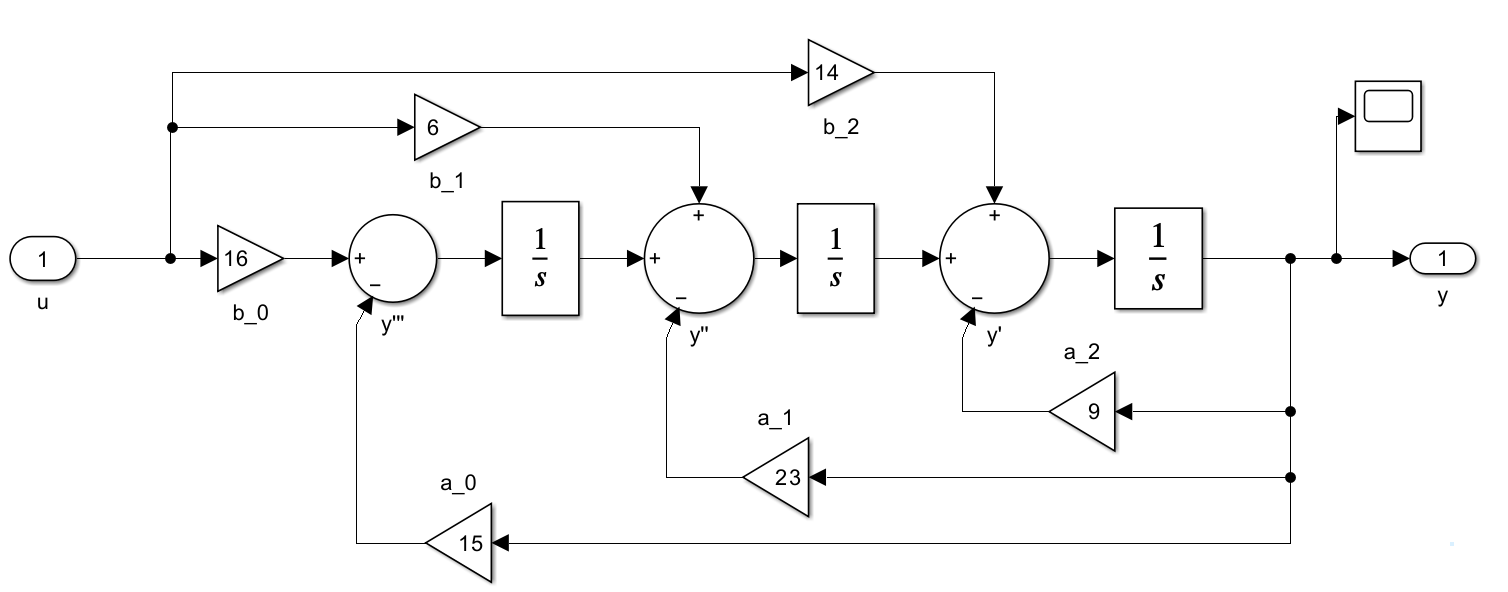
\includegraphics[width=1\linewidth]{pic/schem1.png}}
\caption{Структурная схема первой системы.}
\end{figure}

\newpage
\subsection{Графики сигналов}

\newpage
\section{Задание. Переход от формы вход-выход к форме вход-состояние-выход}





\end{document}













